% \newcommand{\unix}{{\fontspec{Purisa}{UNIX}}}
% \newcommand{\emacs}{\includegraphics[width=1.2em]{emacs-icon}}
% \newcommand{\google}{\raisebox{-.2em}{\includegraphics[width=3em]{google}}}
% \newcommand{\GG}{\textcolor{SkyBlue}{\nerd }}
% \newcommand{\world}{\textcolor{blue}{\nerd }}
\newcommand{\iOS}{\textcolor{orange}{\nerd }}
% \newcommand{\moodle}{
\includegraphics[width=1em]{moodle}}

\title{GNU/Linux}
\author{WANG Xiaolin\\{\footnotesize \texttt{wx672ster+linux@gmail.com}}}

\begin{document}

\frame{\titlepage}

\begin{frame}{Desktop Market Share}{June 2019}
  %http://gs.statcounter.com/os-market-share/desktop/worldwide/#monthly-201906-201906-bar
  \begin{itemize}
  \item[\win] \textcolor{SkyBlue}{\rule{.7843\textwidth}{2mm}}\,
    78.43\%    
  \item[\apple] \textcolor{LightGray}{\rule{.1353\textwidth}{2mm}}\,
    13.53\%
  \item[\linux] \rule{.016\textwidth}{2mm}\, 1.6\%
  \item[\chrome] \textcolor{Orange}{\rule{.0077\textwidth}{2mm}}\,
    0.77\%
  \item[?] \textcolor{Green}{\rule{.0566\textwidth}{2mm}}\, 5.66\%
  \end{itemize}
  \begin{flushright}
    \tiny \url{http://gs.statcounter.com}
  \end{flushright}
  \begin{center}
    \Huge\purisa Why Linux?
  \end{center}
  
  % \begin{tikzpicture}[%
%     every node/.style = {inner sep=0,font=\purisa},%
%     help lines/.style = {ultra thin,dotted},%
%     xy/.style = {font=\ttfamily\tiny,inner sep=1pt},%
%     ]%
%     %%% background image
%     \visible<1->{
%       \node[anchor=south west] (image) at (0,0)%
%       {};%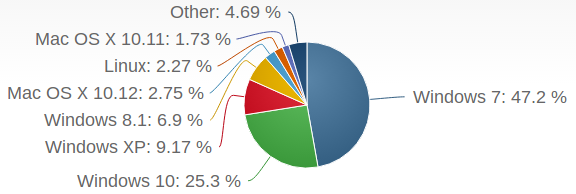
\includegraphics[width=\textwidth]{desktop-marketshare}
%     }
%     \begin{scope}[x={(image.south east)},y={(image.north west)}]%
%       % %%% grid
%       % \draw[help lines,xstep=.1,ystep=.1] (0,0) grid (1,1);%
%       % \foreach \x in {0,1,...,9} { \node [xy,anchor=north] at (\x/10,0) {0.\x}; }%
%       % \foreach \y in {0,1,...,9} { \node [xy,anchor=east] at (0,\y/10) {0.\y}; }%

%       %%% start annotating here %%%
%       \visible<2-3>{\node at (.4,.4)[scale=3,rotate=-30,NavyBlue]  {Why Linux?};}%
%       \visible<3>{\node at (.55,.5) [scale=2,rotate=25,red]%
%         {\textbf{Computer $\neq$ Desktop}};}%
%       \visible<4>{%
%         \node at (.2, .8) [scale=1.5,rotate=30,blue!70] {Desktop};%
%         \node at (.9, .9)[scale=1.5,rotate=-30,violet] {Server};%
%         \node at (.8, .2) [scale=1.5,rotate=25,Green] {Smart Phone};%
%         \node at (.65,.9 ) [scale=1.5,rotate=20,brown] {Tablet};%
%       }
%       \visible<5>{\node at (.5,.5) [scale=5,align=center,red,font=\fontspec{Humor Sans}]%
%         {Everything\\is a\\computer!};}%
%   \end{scope}
% \end{tikzpicture}
\end{frame}

\begin{frame}{OS Market Shares}{June 2019}
  % http://gs.statcounter.com/os-market-share#monthly-201906-201906-bar
  \begin{block}{Everything is a computer}
    PCs, Servers, Smartphones, Tablets...
    \begin{description}
    \item[\android] \textcolor{Green}{\rule{.3961\textwidth}{2mm}}\,
      39.61\%
    \item[\win] \textcolor{SkyBlue}{\rule{.3578\textwidth}{2mm}}\, 35.78\%
    \item[{\iOS}] \textcolor{orange}{\rule{.138\textwidth}{2mm}}\, 13.8\%
    \item[\apple] \textcolor{LightGray}{\rule{.0615\textwidth}{2mm}}\, 6.15\%
    \item[?] \textcolor{gray}{\rule{.0274\textwidth}{2mm}}\, 2.74\%
    \item[\linux] \rule{.0075\textwidth}{2mm}\, 0.75\%
    \item[Other] \textcolor{gray}{\rule{.0117\textwidth}{2mm}}\, 1.17\%
    \end{description}
  \end{block}
  \begin{flushright}
    \tiny \url{http://gs.statcounter.com}
  \end{flushright}
\end{frame}

\begin{frame}{Supercomputer Top500}
  \centering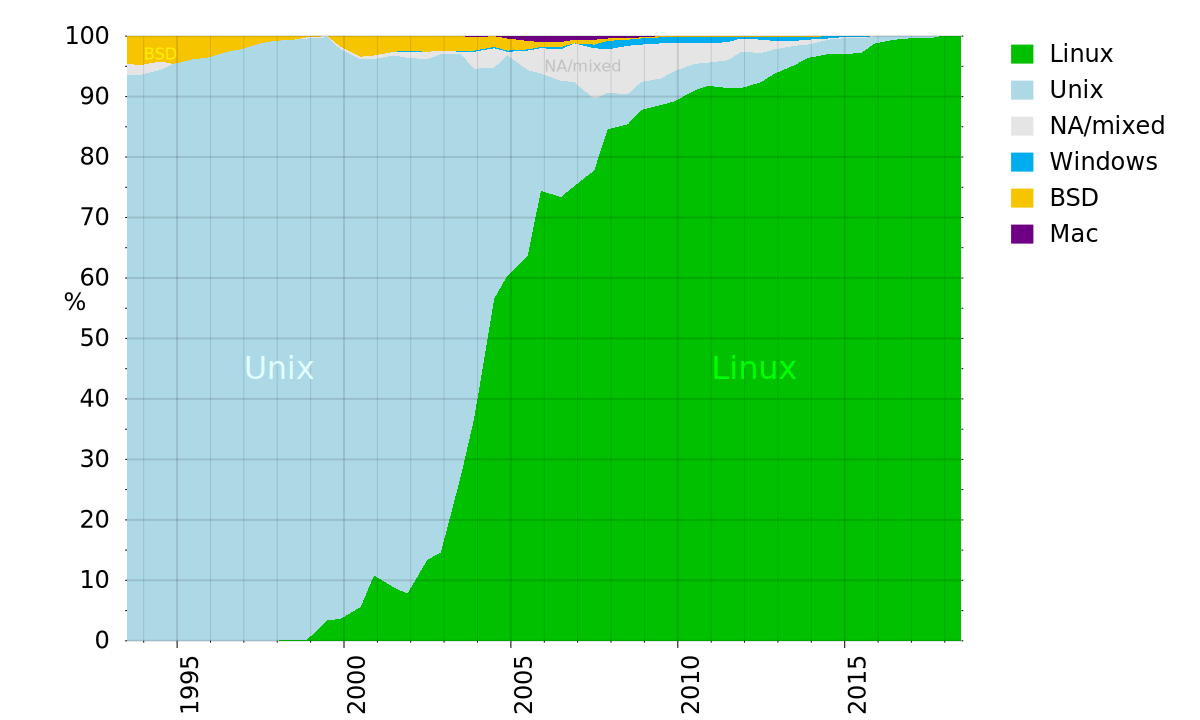
\includegraphics[height=.8\textheight]{top500}
\end{frame}

\begin{frame}{No Textbook}%\openbook
  \begin{itemize}
  \item[\nerd{}] Do you need a book to learn riding a\hspace{.5ex} {\nerd } ?
  \item[{\GG}]\google
    \begin{itemize}{\ttfamily
      \item[\small{\GG}] "linux command line tutorial"
      \item[\small{\GG}] "bash tutorial"
      \item[\small{\GG}] "bash scripting tutorial"
      \item[\small{\GG}] "linux programming tutorial"}
    \end{itemize}
  \item[$\mathbb{E}$] {\purisa English}
  \item[\moodle] \url{https://cs6.swfu.edu.cn/moodle}
  \item[{\small\openbook}] \url{https://cs6.swfu.edu.cn/calibre}
  \end{itemize}
\end{frame}

\begin{frame}{Homework}
  \begin{block}{Weekly tech question}
    \begin{enumerate}
    \item What was I trying to do?
    \item How did I do it? (steps)
    \item The expected output? The real output?
    \item How did I try to solve it? (steps, books, web links)
    \item How many hours did I struggle on it?
    \end{enumerate}
  \end{block}
  \begin{itemize}
  \item[\moodle] \url{https://cs6.swfu.edu.cn/moodle/course/view.php?id=13}
  \item[\Large\dejavu ✉] \alert{\ttfamily wx672ster+linux@gmail.com}
  \item[$\mathbb{E}$] Preferably in English
  \end{itemize}
\end{frame}

\section[History]{A Short History}

\begin{frame}{What's GNU/Linux?}
  \begin{minipage}{.6\textwidth}
    \begin{block}{GNU's Not Unix! --- provides free apps}
      {\Huge\nerd } (GNU's Not Unix!) is a project that was headed by Richard Stallman,
      in 1984, that intended to develop a complete Unix-like operating system that is free
      software.
    \end{block}
    \begin{block}{Linux --- the kernel}
      {\Huge\linux} was written by Linus Torvalds, a graduate student of the University of
      Helsinki in Finland, in early 1990s.
    \end{block}
  \end{minipage}\quad
  \begin{minipage}{.35\textwidth}
    \centering
    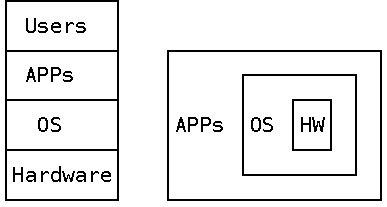
\includegraphics[width=\textwidth]{os}
  \end{minipage}
\end{frame}

\begin{frame}{A Short History of GNU/Linux and Open Source}    
  \begin{description}
  \item[1972:] Ritchie created C language. Unix version 2 written
    mostly by Thompson in C.
  \item[1984:] RMS started the GNU project.
  \item[1985:] FSF was founded by RMS, The GNU manifesto was published.
  \item[1991:] Linux version 0.01 was released on the net.
  \item[1994:] Linux version 1.0 was released.
  \end{description}
\end{frame}

\begin{frame}{Meet The Parents}
  \begin{center}
    \begin{tabularx}{\linewidth}{*{4}{C}}
      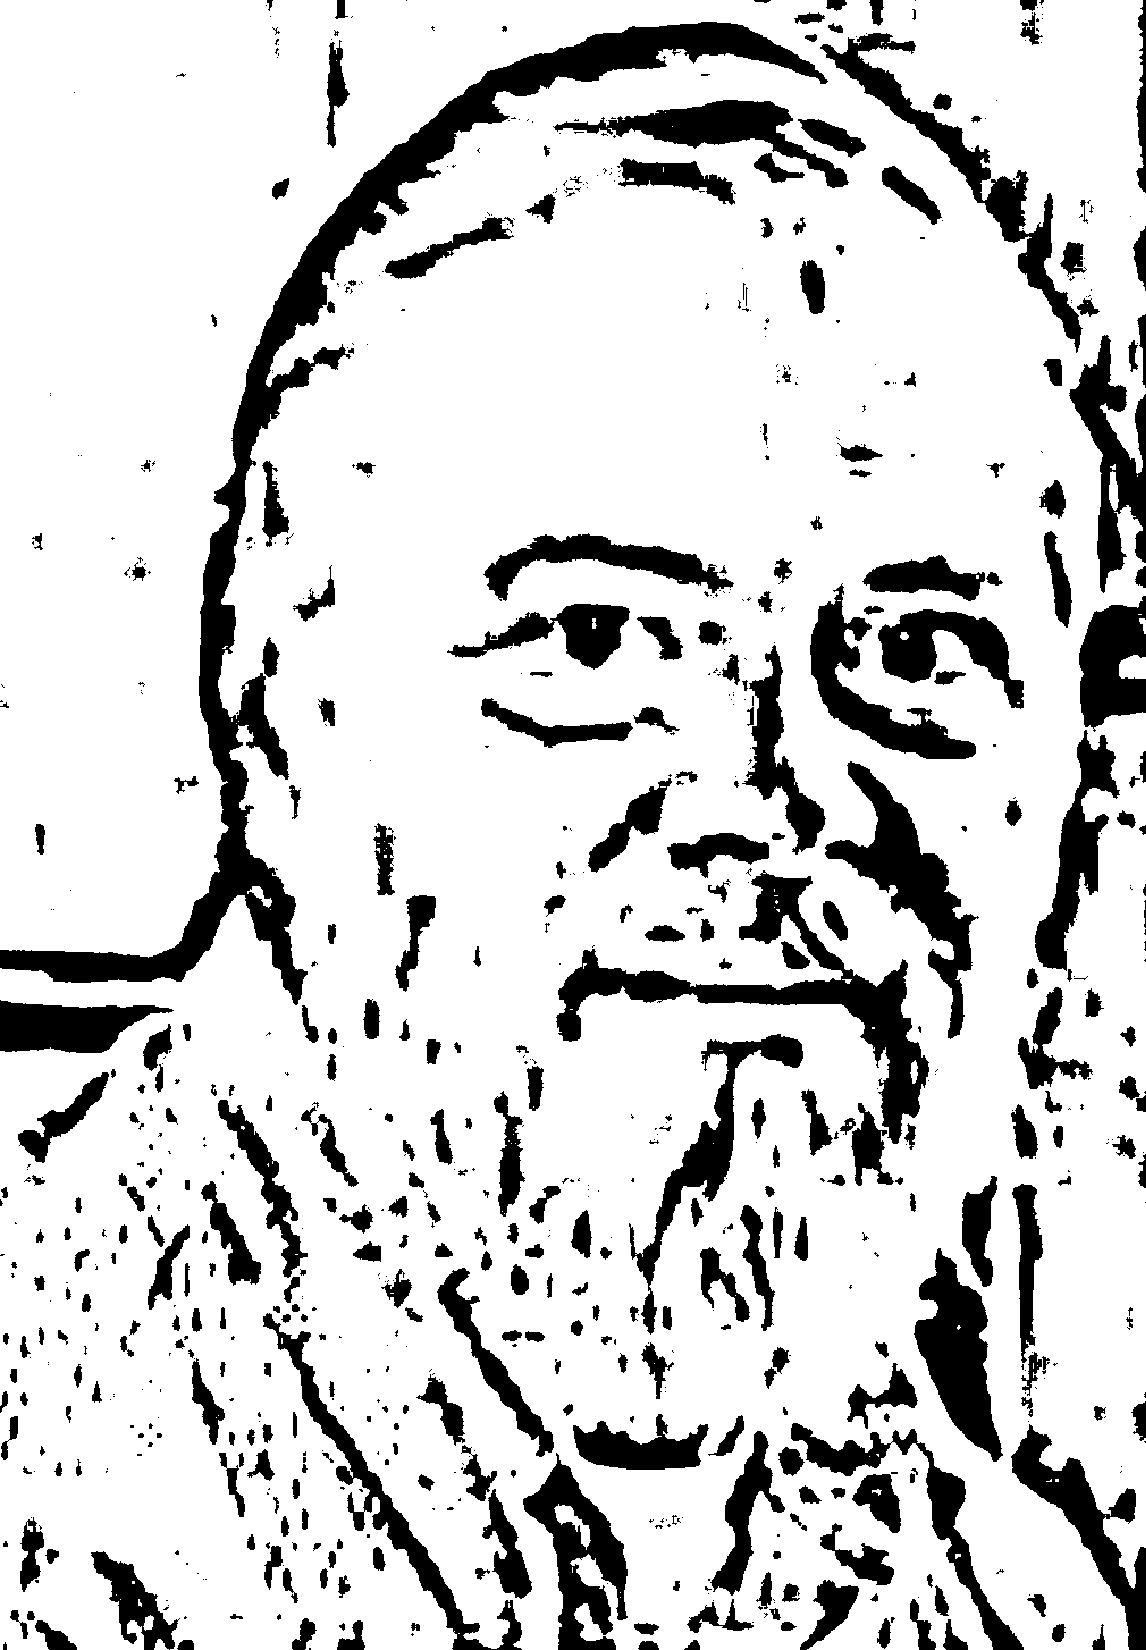
\includegraphics[height=6em]{ritchie}&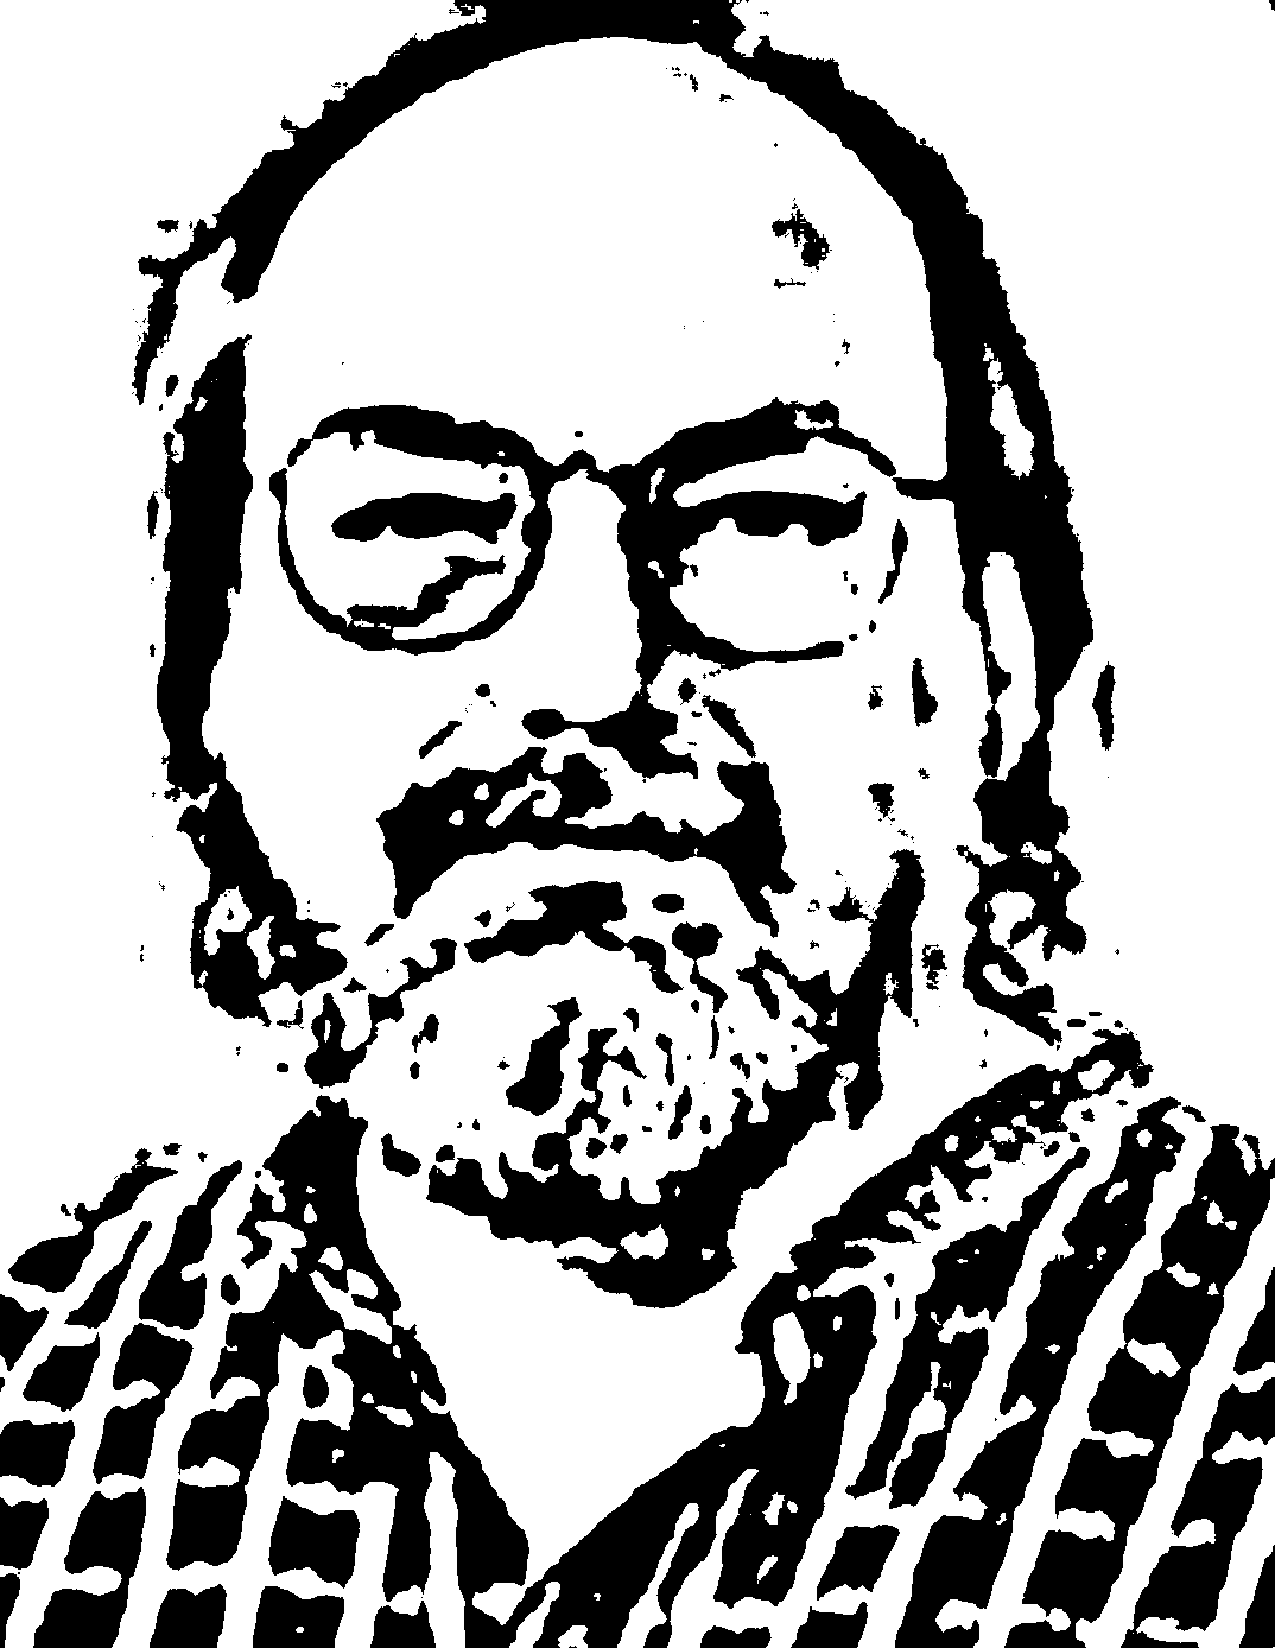
\includegraphics[height=6em]{thompson}&
      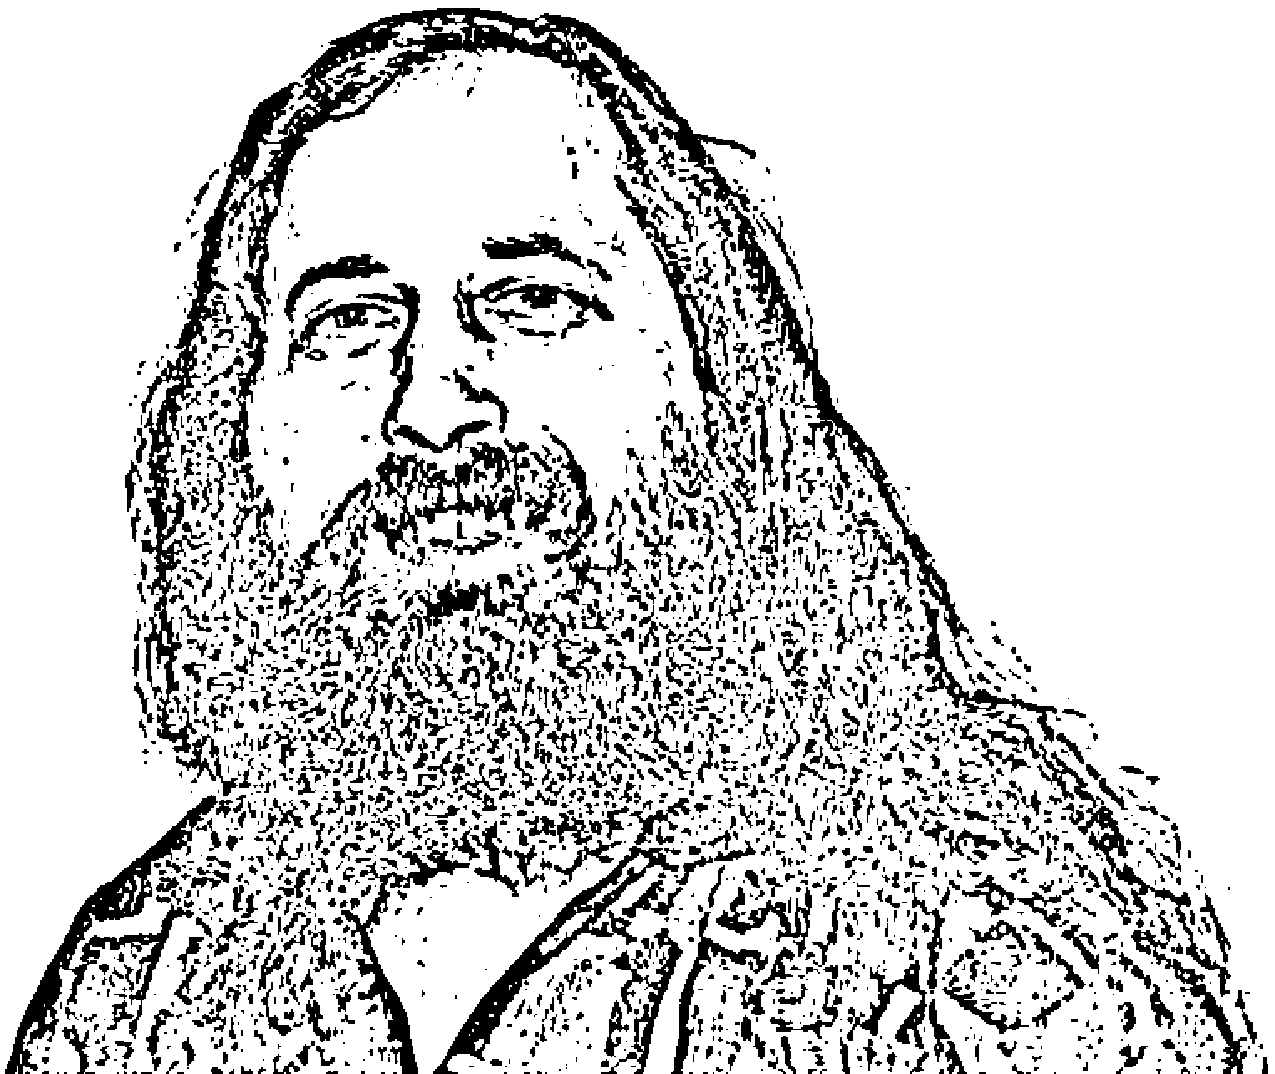
\includegraphics[height=6em]{rms}&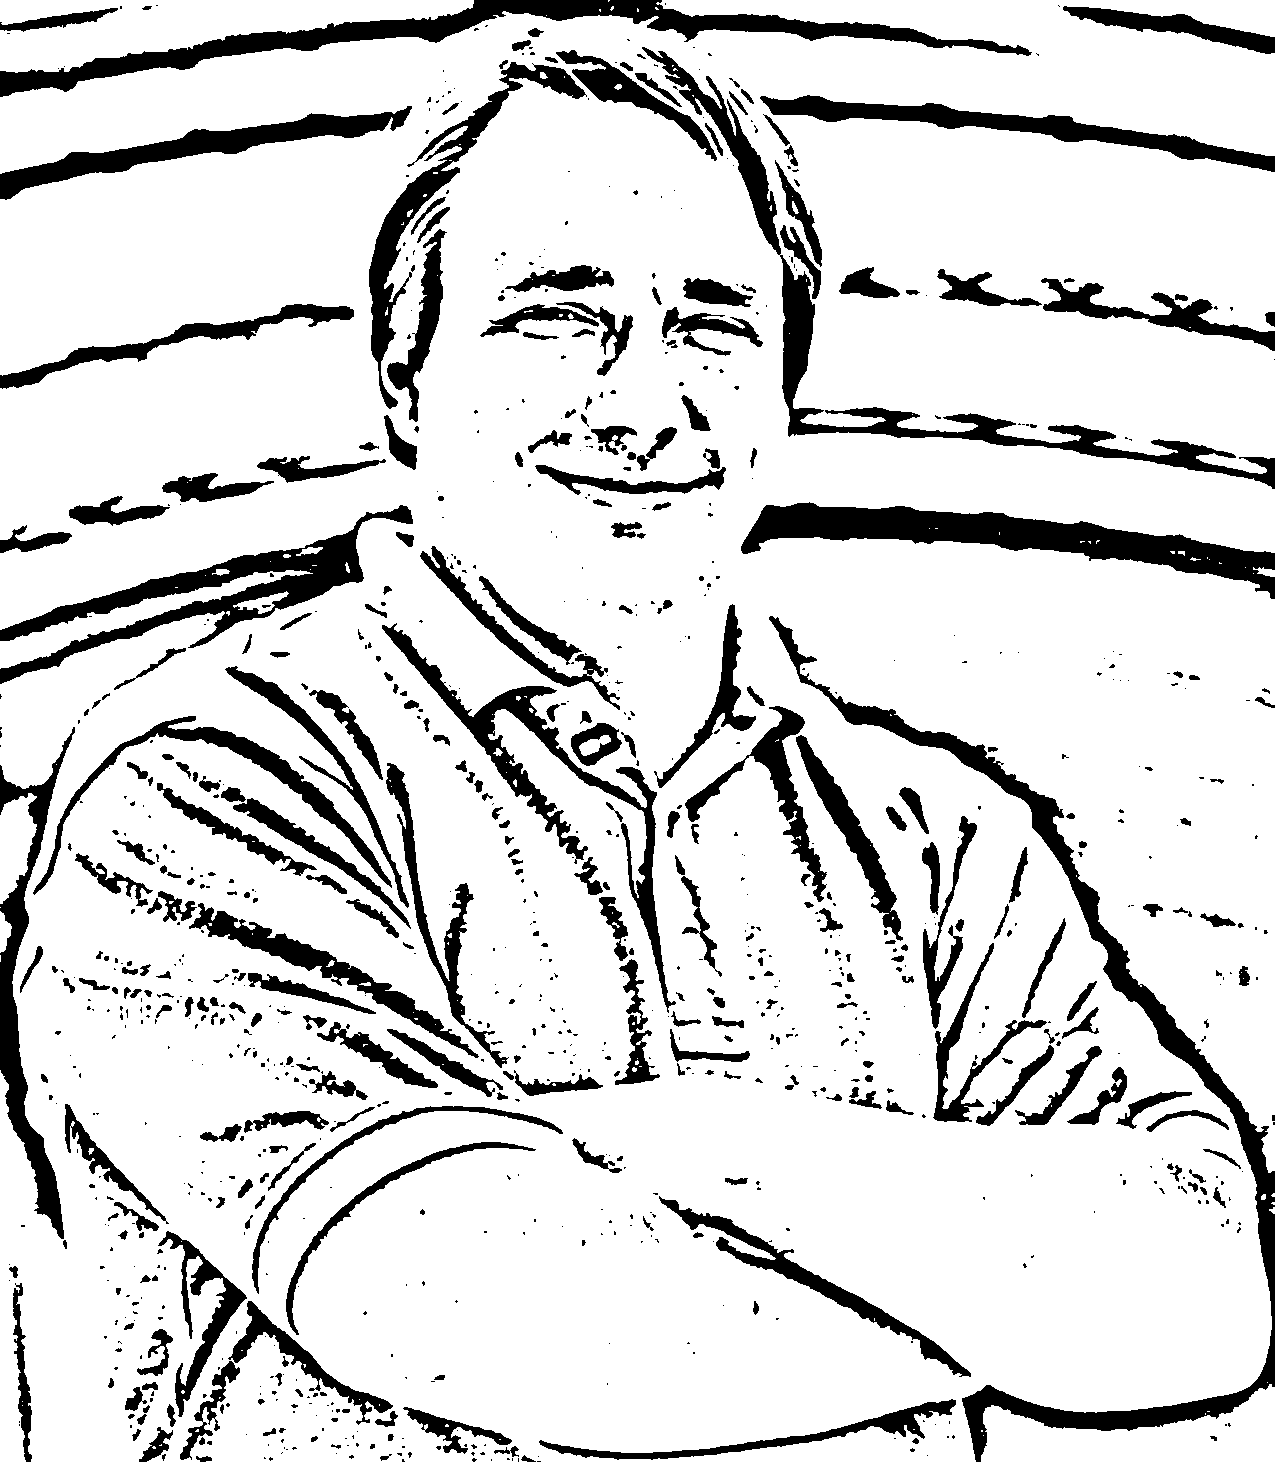
\includegraphics[height=6em]{linus}\\
      {\scriptsize {\purisa Ritche}}&
      {\scriptsize {\purisa Thompson}}&
      {\scriptsize {\purisa RMS}}&
      {\scriptsize {\purisa Linus}}\\
      &&&\\
      \multicolumn{2}{c}{\textbf{\textcolor{gray}{\Huge\unix}}}&
      \scalebox{6.5}{\nerd }&
      \scalebox{5}{\linux}\\
    \end{tabularx}
  \end{center}
\end{frame}

\begin{frame}{How Is GNU/Linux?}
  \centering
  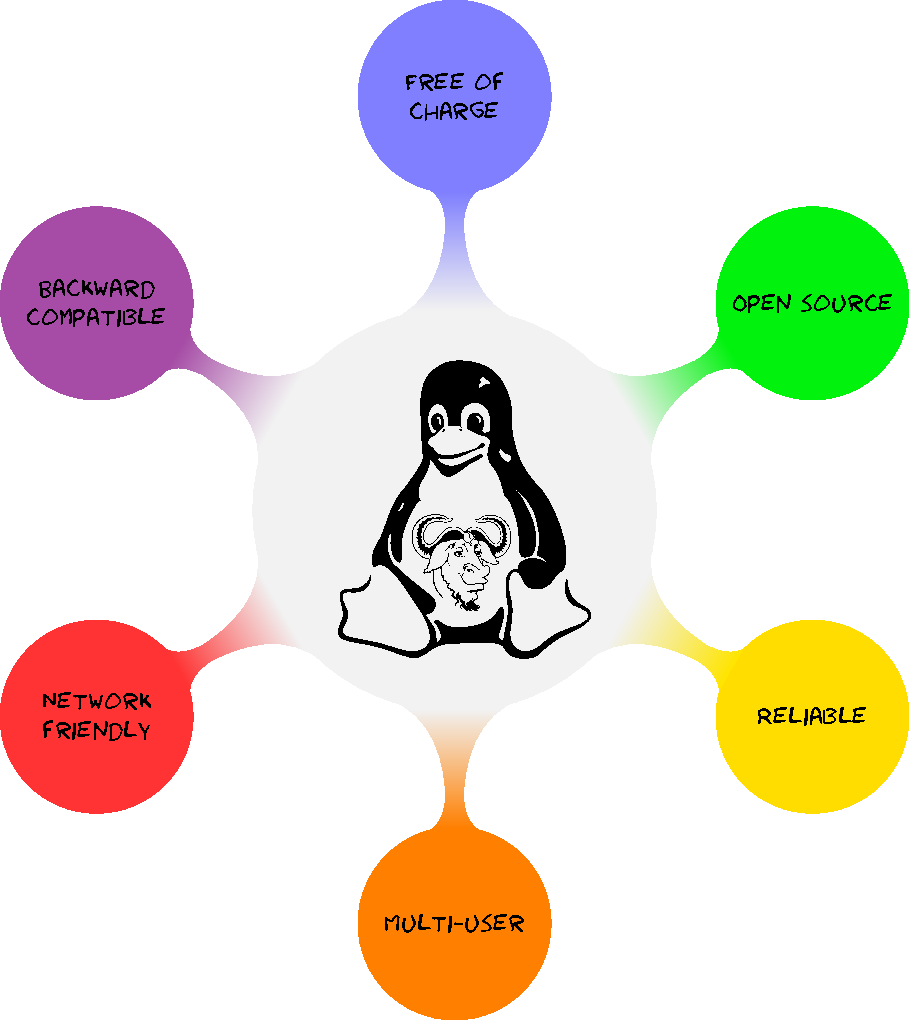
\includegraphics[height=.9\textheight]{pros}
\end{frame}

\section{Open Source}

\begin{frame}{What's Open Source?}
  \begin{description}
  \item[OSI] --- Open Source Initiative
  \item[GPL] --- GNU General Public License, a free, \emph{copyleft} license for software and
    other kinds of works
  \end{description}
  \begin{block}{Share and share alike}
    {\small\purisa ``what you take from the community, you give back.''}
    \begin{itemize}
    \item Free redistribution
    \item Source Code must be included when a modified version is
      released
    \item Derived works follows the same license as of the previous
      works
    \end{itemize}
  \end{block}
\end{frame}

\begin{frame}{Are Companies Into Open Source?}
  \begin{block}{Definitely!}
    \begin{center}
      \includegraphics[width=.5\textwidth]{company}
    \end{center}
  \end{block}
  \begin{description}
  \item[Why?]  Because it benefits them as well.
  \end{description}
\end{frame}

\begin{frame}{The most active companies over the 3.19 to 4.7 development cycles}
  \begin{center}{\small
    \begin{tabular}{@{}l@{}rr|l@{}rr}
      \hline
      \thead{Company} & \thead{Changes} & \thead{Percent} & \thead{Company} & \thead{Changes} & \thead{Percent} \\\hline
      Intel               & 14,384  & 12.9\%  & Outtreachy               & 1,524   & 1.4\%   \\
      RedHat              & 8,987   & 8.0\%   & Vision Engraving Systems & 1,456   & 1.3\%   \\
      \alert{none} & 8,571   & 7.7\%   & Free Electrons           & 1,453   & 1.3\%   \\
      \alert{unknown} & 7,582   & 6.8\%   & NXP Semiconductors       & 1,445   & 1.3\%   \\
      Linaro              & 4,515   & 4.0\%   & Mellanox                 & 1,404   & 1.3\%   \\
      Samsung             & 4,338   & 3.9\%   & Atmel                    & 1,362   & 1.2\%   \\
      SUSE                & 3,619   & 3.2\%   & Broadcom                 & 1,237   & 1.1\%   \\
      IBM                 & 2,995   & 2.7\%   & NVidia                   & 1,146   & 1.0\%   \\
      consultants         & 2,938   & 2.6\%   & Code Aurora Forum        & 1,033   & 0.9\%   \\
      Renesas Electronics & 2,239   & 2.0\%   & Imagination Technologies & 963     & 0.9\%   \\
      Google              & 2,203   & 2.0\%   & Huawei Technologies      & 937     & 0.8\%   \\
      AMD                 & 2,100   & 1.9\%   & Facebook                 & 877     & 0.8\%   \\
      Texas Instruments   & 1,917   & 1.7\%   & Pengutronix              & 790     & 0.7\%   \\
      ARM                 & 1,617   & 1.4\%   & Cisco                    & 692     & 0.6\%   \\
      Oracle              & 1,528   & 1.4\%   & Qualcomm                 & 656     & 0.6\%   \\\hline
    \end{tabular}}
  \end{center}
\end{frame}

\begin{frame}{Linux Development Report 2015}{By Linux foundation}
  \begin{itemize}
  \item Nearly 12,000 developers from more than 1,200 companies have contributed to the
    Linux kernel since tracking began 10 years ago
  \item Just since the last report, more than 4,000 developers from 200 companies have
    contributed to the kernel, half of whom contributed for the first time
  \item The number of paid developers is on the rise, as companies aggressively recruit
    top Linux talent. More than 80\% of kernel development is done by developers who
    are being paid for their work. Volunteer developers tend not to stay that way for long
  \end{itemize}
\end{frame}

\begin{frame}{Why Is It Popular?}
  GNU/Linux presents a \emph{choice}, an alternative to the
  \emph{closed approach} of companies.
  \begin{block}{It's popular among different groups}
    \begin{itemize}
    \item geeks and hobbyists
    \item IT professionals
    \item Software developers
    \item System/Network administrators
    \item Internet/Network engineers
    \end{itemize}
  \end{block}

  \begin{center}
    {\fontspec{Purisa}{In a world without walls and fences, who needs Windows and Gates?}}
  \end{center}
  % \begin{flushright}
  %   --- \raisebox{-1em}{\includegraphics[width=2em]{linux_logo}}
  % \end{flushright}
\end{frame}

\begin{frame}{Is Open Source A Viable Solution?}
  \begin{block}{Yes!}
    \begin{description}
    \item[Apache:] the leading web server in the world\\[1ex]
      {\footnotesize
        \begin{tabular}{rl}
          \textcolor{Red}{Apache}&\textcolor{Red}{\rule{.448\textwidth}{2mm}}\,44.8\%\\
          \textcolor{Green}{Nginx} &\textcolor{Green}{\rule{.401\textwidth}{2mm}}\,40.1\%\\
          \textcolor{Blue}{MS IIS}&\textcolor{Blue}{\rule{.084\textwidth}{2mm}}\,8.4\%\\
          &\makecell[r]{\tiny\emph{(\url{http://W3Techs.com}, 5 July 2019)}}
        \end{tabular}}
    \item[MySQL, PostgreSQL:] popular DBs used among websites
    \item[Perl, PHP, Python:] very hot scripting language% for web development
%    \item[:] the most powerful scripting language in the world
    \item[Sendmail:] the most popular MTA in the world
    \item[BIND:] the most popular DNS server in the world
    \item[GCC:] most popular C/C++ compiler in the world
    \end{description}
  \end{block}
\end{frame}

\section{Facts}

\begin{frame}
  \centering\includegraphics[height=\textheight]{2014}
\end{frame}

\begin{frame}{More Facts}{Popular Web Programming Tools}
  \begin{center}
    \begin{tiny}
      \textbf{ \textcolor{Blue}{ASP}\qquad\qquad \textcolor{Red}{PHP}\qquad\qquad
        \textcolor{Orange}{Python}\qquad\qquad \textcolor{Green}{JSP}\qquad\qquad
        \textcolor{violet}{Ruby}}
    \end{tiny}
  \end{center}
  \begin{center}
    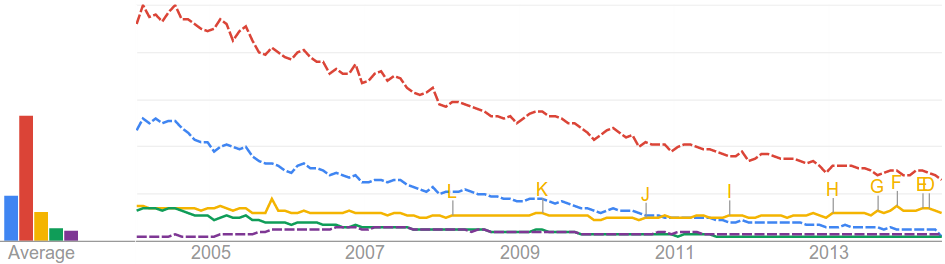
\includegraphics[width=\textwidth]{trends-webp}
  \end{center}
  \centering{
    \textcolor{Red}{PHP},
    \textcolor{Orange}{Python},
    \textcolor{Green}{JSP},
    \textcolor{violet}{Ruby}
    are Linux friendly}
  \vfill
  \flushright{\href{https://www.google.com/trends}{\emph{{\tiny https://www.google.com/trends}}}}
\end{frame}

\begin{frame}{More Facts}{Top10 Programming Languages}
  \begin{center}
    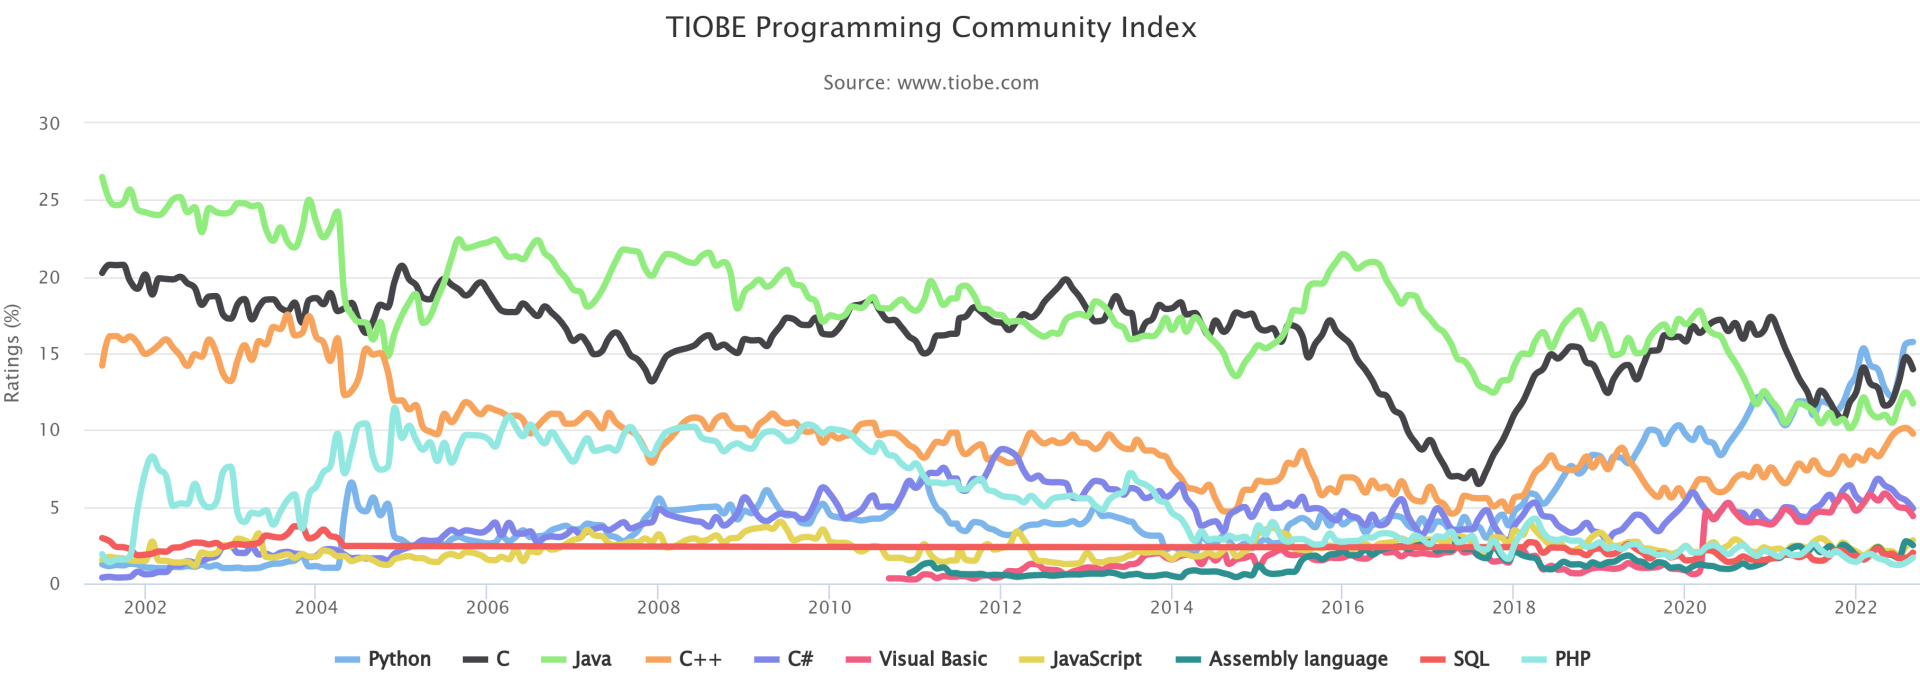
\includegraphics[width=\textwidth]{trends-tiobe}
  \end{center}
  \vfill \flushright{\href{https://www.tiobe.com/tiobe-index//}{\emph{{\tiny TIOBE Index
          for July 2017}}}}
\end{frame}

\begin{frame}{More Facts}{Databases}
  \begin{center}
    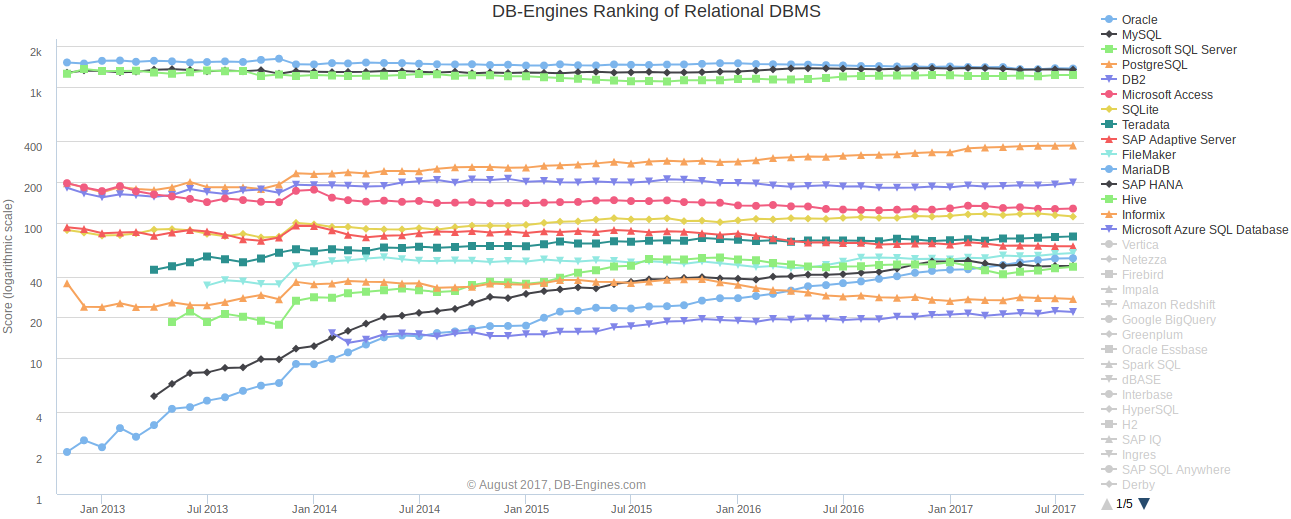
\includegraphics[width=\textwidth]{db-ranking}
  \end{center}
  \vfill
  \flushright{\href{http://db-engines.com/en/ranking_trend/relational+dbms}{{\tiny
        \emph{DB-Engines Ranking --- Trend of Relational DBMS Popularity}}}} 
\end{frame}

\begin{frame}{Smartphone Market Share}
  \begin{center}
    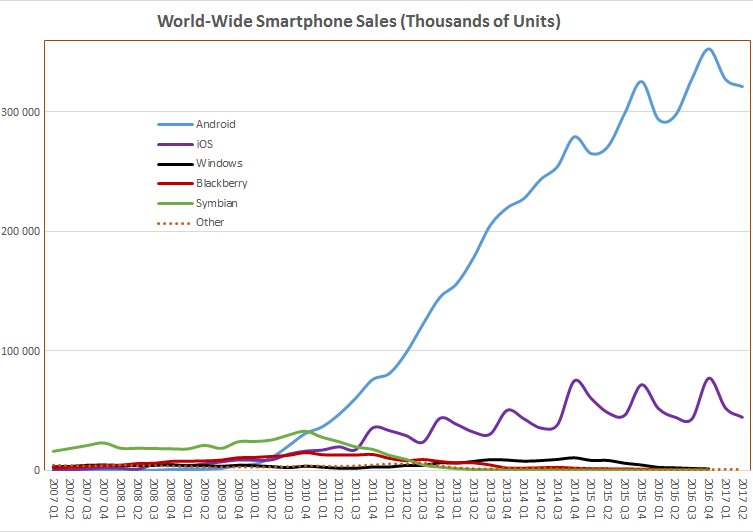
\includegraphics[height=.7\textheight]{smartphone-share}
  \end{center}
  {\footnotesize
  \begin{itemize}
  \item[\android] \textcolor{Green}{\rule{.8\textwidth}{2mm}}\, 86.1\%
  \item[\apple] \textcolor{LightGray}{\rule{.137\textwidth}{2mm}}\, 13.7\%
  \item[Other] \textcolor{gray}{\rule{.002\textwidth}{2mm}}\, 0.2\%
  \end{itemize}}
\end{frame}

\begin{frame}{Games}
  \begin{columns}
    \begin{column}{.5\textwidth}
      \begin{block}{Steam platform support}
        \begin{itemize}
        \item[\win] since 2002
        \item[\apple] since 2010
        \item[\linux] since July, 2012
        \end{itemize}
      \end{block}
    \end{column}
    \begin{column}{.5\textwidth}
      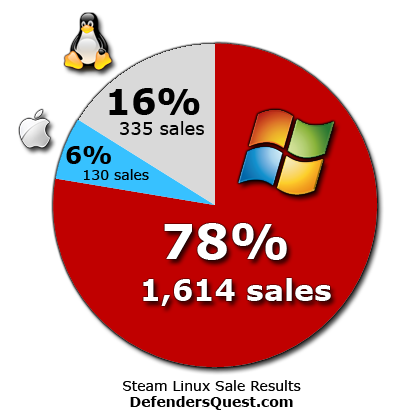
\includegraphics[width=\textwidth]{steam_linux_piechart}      
    \end{column}
  \end{columns}
\end{frame}

\begin{frame}{Use The Right Tools For The Right Jobs}
  \begin{block}{I don't mean\,\linux\,is for everyone to do everything}
    \begin{itemize}
    \item \win\, is the platform of choice for audio enthusiasts and
      gamers
    \item \apple\, are the choice for most graphics designers, desktop
      publishing firms, and video production houses
    \item SGI is king when it comes to 3D modelling/animation
    \item Solaris and other commercial Unices have there place in the world
    \end{itemize}
  \end{block}
\end{frame}

% \begin{frame}{The Distance}{
\includegraphics[width=2em]{ie}}
%   \begin{center}
%     \includegraphics[width=\textwidth]{ie6}
%   \end{center}
% \end{frame}

\begin{frame}{The Distance}% Between China And The World}
  \begin{center}
    \begin{tabular}{cc}
      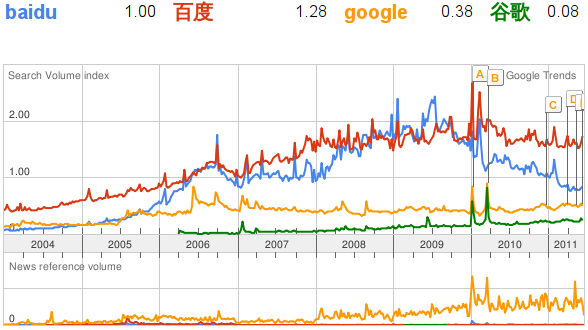
\includegraphics[width=.5\textwidth]{search-cn-trends}&% 
      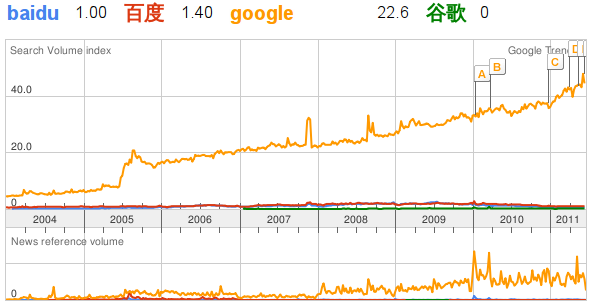
\includegraphics[width=.5\textwidth]{search-trends}\\
      
\includegraphics[width=2em]{china-f}&{\Huge\world}
    \end{tabular}
  \end{center}
\end{frame}

\section{How to learn}

\begin{frame}{How To Learn GNU/Linux?}
  \begin{block}{My advices}
    \begin{itemize}
    \item Use \,{\linux}\, to do your daily work. Can you do...
      \begin{itemize}
      \item[-] homework on \linux?
      \item[-] coding on \linux?
      \item[-] lab work on \linux?
        \begin{itemize}
        \item[if] \textbf{\textcolor{Red}{\purisa NO}}
        \item[then] Start \textbf{\textcolor{Red}{\purisa NOW!}}
        \end{itemize}
      \end{itemize}
    \item {\nerd } \world
      \begin{itemize}
      \item[-] \google
      \item[-] {\purisa English}
      \end{itemize}
    \end{itemize}
  \end{block}
\end{frame}

\begin{frame}{Which Distribution?}
  \begin{minipage}{.35\linewidth}
    \includegraphics[width=\textwidth]{Gldt}
  \end{minipage}\quad
  \begin{minipage}{.55\linewidth}
    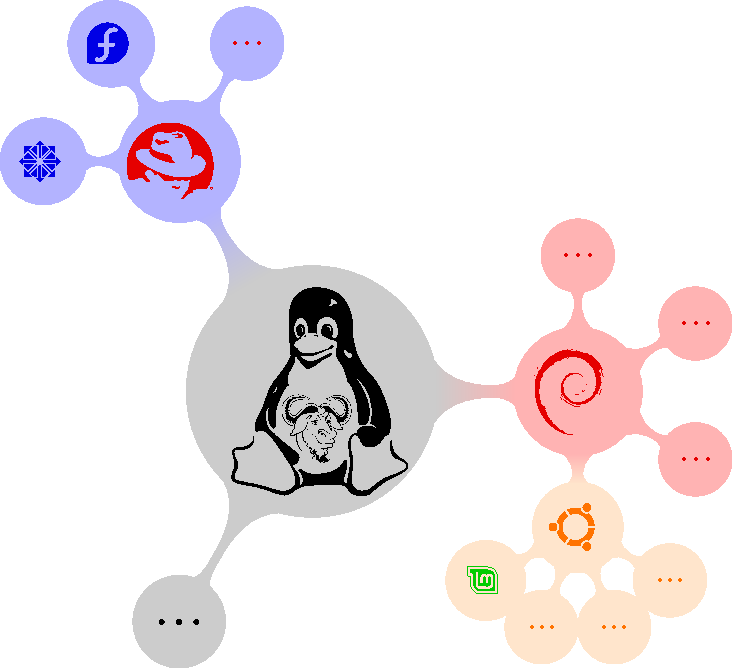
\includegraphics[width=\textwidth]{map}
  \end{minipage}
\end{frame}

% \begin{frame}{References}
%   \begin{itemize}
%   \item \href{http://www.opensource.org/}{Open Source Initiative}
%   \item \href{http://www.gnu.org}{GNU Project}
%   \item \href{http://www.linux.org/}{Linux Online}
%   \item \href{http://www.linuxlinks.com}{LinuxLinks.com}
%   \end{itemize}
% \end{frame}

\end{document}

%%% Local Variables:
%%% mode: latex
%%% TeX-master: "linux_intro-b"
%%% End:
